\documentclass[dvisvgm,border=2mm]{standalone}
\usepackage[T1]{fontenc}
\usepackage{amsmath,amssymb,bm}
\usepackage{mathptmx}
\usepackage{tikz}
\usetikzlibrary{arrows.meta,positioning}

\begin{document}
% DAG 2 — the one line that differs: observed count vs censored left tail.
% Shaded = observed ; dashed = latent (the count we never see).
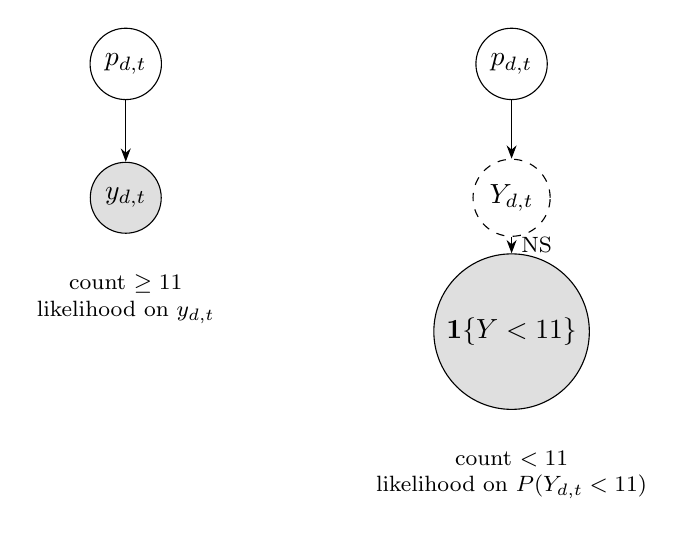
\begin{tikzpicture}[>=Stealth, node distance=1.7cm]
  % left: an observed cell
  \node[circle, draw] (p1) {$p_{d,t}$};
  \node[circle, draw, fill=gray!25, below of=p1] (y1) {$y_{d,t}$};
  \draw[->] (p1) -- (y1);
  \node[font=\footnotesize, below=0.4cm of y1, align=center] {count $\ge 11$\\ likelihood on $y_{d,t}$};

  % right: a suppressed cell
  \node[circle, draw, right of=p1, xshift=3.2cm] (p2) {$p_{d,t}$};
  \node[circle, draw, dashed, below of=p2] (Y2) {$Y_{d,t}$};
  \node[circle, draw, fill=gray!25, below of=Y2] (ns) {$\mathbf{1}\{Y<11\}$};
  \draw[->] (p2) -- (Y2);
  \draw[->] (Y2) -- (ns) node[midway, right, font=\footnotesize] {NS};
  \node[font=\footnotesize, below=0.4cm of ns, align=center] {count $< 11$\\ likelihood on $P(Y_{d,t}<11)$};
\end{tikzpicture}
\end{document}
